\chapter{Arhitektura i dizajn sustava}
		
	\vspace{-1cm}
	\begin{figure}[h]
		\begin{center}
			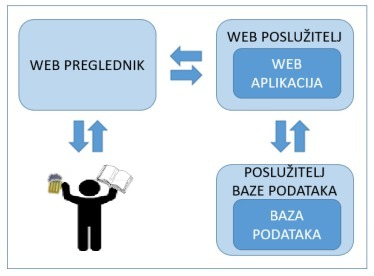
\includegraphics{slike/arhitektura_skica.png}
			\caption{Arhitektura sustava}
		\end{center}	
	\end{figure}
	
	\indent Arhitekturu tvore tri podsustava: web poslužitelj, web aplikacija te baza podataka. \textit{Web preglednik} je program za pregledavanje i navigaciju web-stranicama. Kada korisnik pošalje zahtjev za web-stranicom, preglednik dohvaća potrebne datoteke s \textit{web poslužitelja} i prikazuje stranicu na korisnikovom ekranu u namijenjenom obliku. Poslužitelj omogućuje komunikaciju klijenta s \textit{web aplikacijom} koja je na njemu pokrenuta, a prosljeđuje joj zahtjeve HTTP-om (engl. \textit{Hyper Text Transfer Protocol}). Web aplikacija odgovara na zahtjeve klijenta pristupajući po potrebi bazi podataka i vraćajući HTML dokument čitljiv u web pregledniku. \\
	
	\indent Za izradu ovog projekta koristili smo se Spring Boot frameworkom u Javi kroz razvojno okruženje IntelliJ Community Edition, Javascriptom uz React u Visual Studio Code-u te nizom drugih programa za dizajn slika i grafova (GIMP, AstahUML itd.). \\
	
	\indent Arhitektura sustava prati MVC obrazac, odnosno Model-Pogled-Nadglednik (engl. \textit{Model View Controller}), stilističku varijaciju arhitekture zasnovane na događajima. Takve arhitekture odlikuje to što se komponente međusobno ne pozivaju eksplicitno, već neke od njih generiraju signale (događaje) ne znajući koja druga "osluškuje" tj. očekuje takav signal i na njega reagira. Kod MVC-a pogodno je što smanjuje međuovisnost korisničkog sučelja i ostatka sustava, a omogućuje i nezavisan razvoj, nadogradnje i dodavanje različitih dijelova aplikacije. Sadrži različite gotove predloške za klase koji nam olakšavaju proces izrade.\\
	
	\indent MVC model sastoji se od komponenti:
	\begin{packed_item}
		\item 	\textbf{Model} - Središnja komponenta sustava, sadrži razrede čiji se objekti obrađuju. Rukuje s podatkovnom logikom i bazom podataka. Prima podatke od nadglednika.
		\item 	\textbf{Pogled} - Predstavlja model korisniku na čitljiv način. Sadrži razrede čiji objekti služe za prikaz podataka. Dinamički se osvježava.
		\item	\textbf{Nadglednik} - Razumije naputke korisnika i pretvara ih u upute ka modelu. Sadrži razrede koji upravljaju i rukuju korisničkom interakcijom s pogledom i modelom, poput poslovne logike i odgovora na događaje.
	\end{packed_item}

	\eject
		

		

				
		\section{Baza podataka}
			
			\textbf{\textit{dio 1. revizije}}\\
			
		\textit{Potrebno je opisati koju vrstu i implementaciju baze podataka ste odabrali, glavne komponente od kojih se sastoji i slično.}
		
		Za potrebe našeg sustava koristit ćemo relacijsku bazu podataka koja svojom strukturom olakšava modeliranje stvarnog svijeta. Gradivna jedinka baze je relacija, odnosno tablica koja je definirana svojim imenom i skupom atributa. Zadaća baze podataka je brza i jednostavna pohrana, izmjena i dohvat podataka za daljnju obradu.Baza podataka ove aplikacije sastoji se od sljedećih entiteta:
		
		\begin{itemize}
			\item Korisnik
			\item Uloga
			\item Vrsta
			\item Oznaka
			\item ImaUlogu
			\item JePrijatelj
			\item JeBlokiranOd
			\item Dogadjaj
			\item Pohadja
			\item ImaOznaku
			
		\end{itemize}
		
		
			\subsection{Opis tablica}
			

				\textit{Svaku tablicu je potrebno opisati po zadanom predlošku. Lijevo se nalazi točno ime varijable u bazi podataka, u sredini se nalazi tip podataka, a desno se nalazi opis varijable. Svjetlozelenom bojom označite primarni ključ. Svjetlo plavom označite strani ključ}
				
				\noindent\textbf{Korisnik} Ovaj entitet sadržava sve važne informacije o korisniku aplikacije. Sadrži atribute: id korisnika, nadimak, korisničko ime, email, salt, lozinka i suspendiran.
				
				\begin{longtblr}[
					label=none,
					entry=none
					]{
						width = \textwidth,
						colspec={|X[6,l]|X[6, l]|X[20, l]|}, 
						rowhead = 1,
					} %definicija širine tablice, širine stupaca, poravnanje i broja redaka naslova tablice
					\hline \multicolumn{3}{|c|}{\textbf{Korisnik}}	 \\ \hline[3pt]
					\SetCell{LightGreen}id korisnik & BIGINT NOT NULL	&  	Lorem ipsum dolor sit amet, consectetur adipiscing elit, sed do eiusmod  	\\ \hline
					nadimak	& VARCHAR(25) NOT NULL &   	\\ \hline
					korisnicko ime & VARCHAR(25) NOT NULL &   \\ \hline  
					email & VARCHAR(255) NOT NULL &   \\ \hline 
					salt & BYTEA NOT NULL	&  		\\ \hline 
					lozinka & BYTEA NOT NULL	&  		\\ \hline 
					suspendiran & BOOLEAN NOT NULL	&  		\\ \hline 
					
				\end{longtblr}
			
			
				\noindent\textbf{Uloga} Ovaj entitet sadržava sve važne informacije o ulogama korisnika. Sadrži atribute: id uloga, naziv uloga i opis uloga.
				
				\begin{longtblr}[
					label=none,
					entry=none
					]{
						width = \textwidth,
						colspec={|X[6,l]|X[6, l]|X[20, l]|}, 
						rowhead = 1,
					} %definicija širine tablice, širine stupaca, poravnanje i broja redaka naslova tablice
					\hline \multicolumn{3}{|c|}{\textbf{Uloga}}	 \\ \hline[3pt]
					\SetCell{LightGreen}id uloga & BIGINT NOT NULL	&  	Lorem ipsum dolor sit amet, consectetur adipiscing elit, sed do eiusmod  	\\ \hline
					naziv uloga	& VARCHAR(255) NOT NULL &   	\\ \hline 
					opis uloga & VARCHAR(255) NOT NULL &   \\ \hline 
					
				\end{longtblr}
			
				\noindent\textbf{Vrsta} Ovaj entitet sadržava sve važne informacije o vrstama događaja. Sadrži atribute: id vrsta, naziv vrsta i opis vrsta.
				
				\begin{longtblr}[
					label=none,
					entry=none
					]{
						width = \textwidth,
						colspec={|X[6,l]|X[6, l]|X[20, l]|}, 
						rowhead = 1,
					} %definicija širine tablice, širine stupaca, poravnanje i broja redaka naslova tablice
					\hline \multicolumn{3}{|c|}{\textbf{Vrsta}}	 \\ \hline[3pt]
					\SetCell{LightGreen}id vrsta & INT NOT NULL	&  	Lorem ipsum dolor sit amet, consectetur adipiscing elit, sed do eiusmod  	\\ \hline
					naziv vrsta	& VARCHAR(255) NOT NULL &   	\\ \hline 
					opis vrsta & VARCHAR(255) NOT NULL &   \\ \hline 
					 
				\end{longtblr}
				
				\noindent\textbf{Oznaka} Ovaj entitet sadržava sve važne informacije o oznakama događaja. Sadrži atribute: id oznaka, naziv oznaka i boja hex.
				
				\begin{longtblr}[
					label=none,
					entry=none
					]{
						width = \textwidth,
						colspec={|X[6,l]|X[6, l]|X[20, l]|}, 
						rowhead = 1,
					} %definicija širine tablice, širine stupaca, poravnanje i broja redaka naslova tablice
					\hline \multicolumn{3}{|c|}{\textbf{Oznaka}}	 \\ \hline[3pt]
					\SetCell{LightGreen}id oznaka & INT NOT NULL	&  	Lorem ipsum dolor sit amet, consectetur adipiscing elit, sed do eiusmod  	\\ \hline
					naziv oznaka	& VARCHAR(255) NOT NULL &   	\\ \hline 
					boja hex & CHAR(7) NOT NULL &   \\ \hline 
					
				\end{longtblr}
				
				
				\noindent\textbf{ImaUlogu} Ovaj entitet sadržava sve važne informacije po kojima saznajemo koji korisnik ima koju ulogu. Sadrži atribute: id korisnik i id uloga.
				
				\begin{longtblr}[
					label=none,
					entry=none
					]{
						width = \textwidth,
						colspec={|X[6,l]|X[6, l]|X[20, l]|}, 
						rowhead = 1,
					} %definicija širine tablice, širine stupaca, poravnanje i broja redaka naslova tablice
					\hline \multicolumn{3}{|c|}{\textbf{ImaUlogu}}	 \\ \hline[3pt]
					\SetCell{LightGreen}id korisnik & BIGINT NOT NULL	&  	Lorem ipsum dolor sit amet, consectetur adipiscing elit, sed do eiusmod  	\\ \hline
					\SetCell{LightGreen}id uloga	& BIGINT NOT NULL &   	\\ \hline 
					 
				\end{longtblr}
				
				\noindent\textbf{JePrijatelj} Ovaj entitet sadržava sve važne informacije o tome koji je korisnik nekom drugom korisniku prijatelj. Sadrži atribute: id korisnik i id prijatelj.
				
				\begin{longtblr}[
					label=none,
					entry=none
					]{
						width = \textwidth,
						colspec={|X[6,l]|X[6, l]|X[20, l]|}, 
						rowhead = 1,
					} %definicija širine tablice, širine stupaca, poravnanje i broja redaka naslova tablice
					\hline \multicolumn{3}{|c|}{\textbf{JePrijatelj}}	 \\ \hline[3pt]
					\SetCell{LightGreen}id korisnik & BIGINT NOT NULL	&  	Lorem ipsum dolor sit amet, consectetur adipiscing elit, sed do eiusmod  	\\ \hline
					\SetCell{LightGreen}id prijatelj	& BIGINT NOT NULL	& 	\\ \hline 
				\end{longtblr}
			
			
				\noindent\textbf{JeBlokiranOd} Ovaj entitet sadržava sve važne informacije o tome koji je korisnik blokiran i od kojeg je korisnika blokiran. Sadrži atribute: id blokiran i id blokiran od.
				
				\begin{longtblr}[
					label=none,
					entry=none
					]{
						width = \textwidth,
						colspec={|X[6,l]|X[6, l]|X[20, l]|}, 
						rowhead = 1,
					} %definicija širine tablice, širine stupaca, poravnanje i broja redaka naslova tablice
					\hline \multicolumn{3}{|c|}{\textbf{JeBlokiranOd}}	 \\ \hline[3pt]
					\SetCell{LightGreen}id blokiran & BIGINT NOT NULL	&  	Lorem ipsum dolor sit amet, consectetur adipiscing elit, sed do eiusmod  	\\ \hline
					\SetCell{LightGreen}id blokiran od	& BIGINT NOT NULL &   	\\ \hline 
				 
				\end{longtblr}
				
				
				\noindent\textbf{Dogadjaj} Ovaj entitet sadržava sve važne informacije o događaju. Sadrži atribute: id događaj, naziv, mjesto, vrijeme početka, vrijeme kraja, opis, promoviran, koordinate, id organizator i id vrsta.
				
				\begin{longtblr}[
					label=none,
					entry=none
					]{
						width = \textwidth,
						colspec={|X[6,l]|X[6, l]|X[20, l]|}, 
						rowhead = 1,
					} %definicija širine tablice, širine stupaca, poravnanje i broja redaka naslova tablice
					\hline \multicolumn{3}{|c|}{\textbf{Dogadjaj}}	 \\ \hline[3pt]
					\SetCell{LightGreen}id dogadjaj & BIGINT NOT NULL	&  	Lorem ipsum dolor sit amet, consectetur adipiscing elit, sed do eiusmod  	\\ \hline
					naziv	& VARCHAR(255) NOT NULL &   	\\ \hline 
					mjesto & VARCHAR(255) NOT NULL &   \\ \hline 
					vrijeme poc & TIMESTAMP NOT NULL	&  		\\ \hline 
					vrijeme kraj & TIMESTAMP NOT NULL	&  		\\ \hline
					opis & VARCHAR(255) NOT NULL &  \\ \hline
					promoviran & BOOLEAN NOT NULL &   \\ \hline 
					koordinate & VARCHAR(255) NOT NULL &  \\ \hline
					\SetCell{LightBlue}id organizator & BIGINT NOT NULL &   \\ \hline 
					\SetCell{LightBlue}id vrsta & INT NOT NULL & 
					\\ \hline
				\end{longtblr}
				
				
				\noindent\textbf{Pohadja} Ovaj entitet sadržava sve važne informacije o tome tko je pohađao koji događaj i kako ga je ocijenio. Sadrži atribute: recenzija, id polaznika i id događaja.
				
				\begin{longtblr}[
					label=none,
					entry=none
					]{
						width = \textwidth,
						colspec={|X[6,l]|X[6, l]|X[20, l]|}, 
						rowhead = 1,
					} %definicija širine tablice, širine stupaca, poravnanje i broja redaka naslova tablice
					\hline \multicolumn{3}{|c|}{\textbf{Pohadja}}	 \\ \hline[3pt]
					recenzija & SMALLINT NOT NULL	&  	Lorem ipsum dolor sit amet, consectetur adipiscing elit, sed do eiusmod  	\\ \hline
				    \SetCell{LightGreen} id pohadjatelja	& BIGINT NOT NULL &   	\\ \hline 
					\SetCell{LightGreen} id dogadjaja & BIGINT NOT NULL &   \\ \hline 
					 
				\end{longtblr}
			
				
				\noindent\textbf{ImaOznaku} Ovaj entitet sadržava sve važne informacije o oznakama određenih događaja. Sadrži atribute: id događaj i id oznaka.
				
				\begin{longtblr}[
					label=none,
					entry=none
					]{
						width = \textwidth,
						colspec={|X[6,l]|X[6, l]|X[20, l]|}, 
						rowhead = 1,
					} %definicija širine tablice, širine stupaca, poravnanje i broja redaka naslova tablice
					\hline \multicolumn{3}{|c|}{\textbf{ImaOznaku}}	 \\ \hline[3pt]
					\SetCell{LightGreen}id dogadjaj & BIGINT NOT NULL	&  	Lorem ipsum dolor sit amet, consectetur adipiscing elit, sed do eiusmod  	\\ \hline
					\SetCell{LightGreen}id oznaka	& INT NOT NULL &   	\\ \hline 
				
				\end{longtblr}
			
				
			
			
				
				
			
			\subsection{Dijagram baze podataka}
				
				
			\begin{figure}[h]
				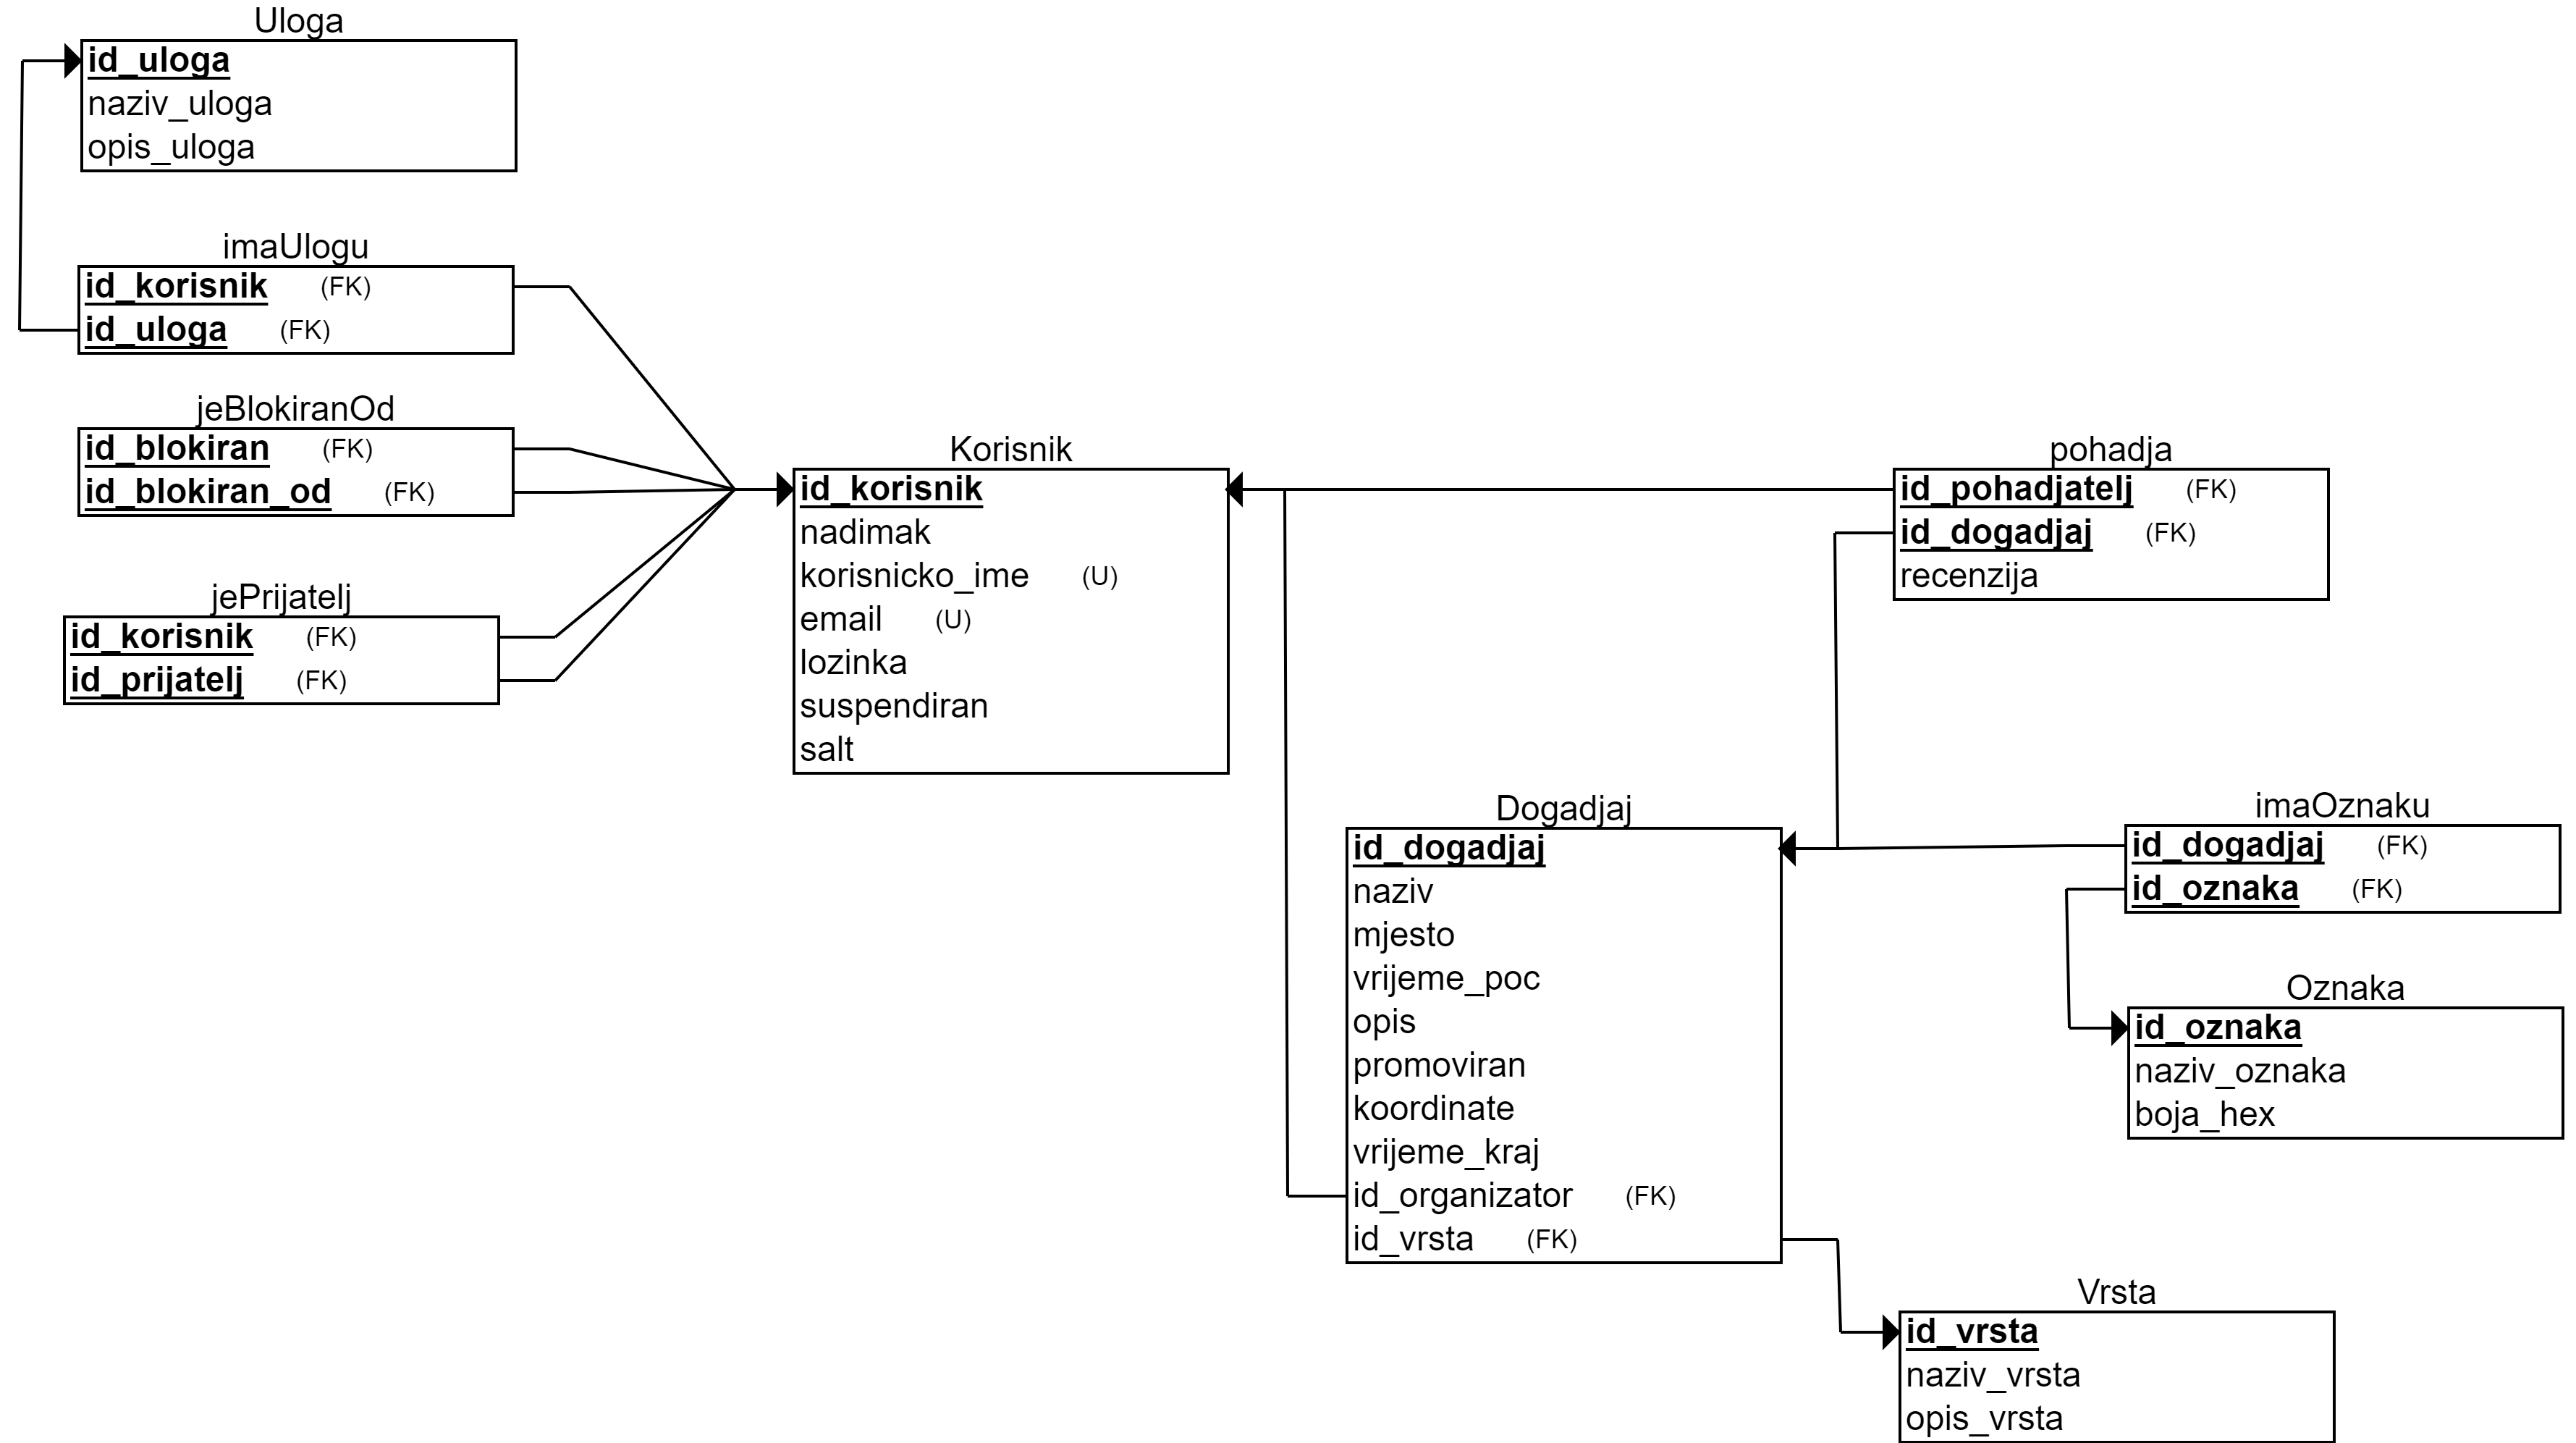
\includegraphics[width=\textwidth]{dijagrami/Baza podataka/REL shema.png}
				\caption{E-R dijagram baze podataka}
			\end{figure}
				
			\eject
			
			
		\section{Dijagram razreda}
			
			\indent Na naredne tri slike nalaze se dijagrami razreda podijeljeni logički po srodnosti. Neki razredi povezani su i s onima na odvojenim slikama što se da zaključiti po nazivima njihovih metoda. \\
			
			\indent Razredi na slici 4.4 uokvireni plavom bojom su controlleri. Njihove metode služe za primanje i slanje DTO-ova (\textit{Data Transfer Objects})  prema frontendu u obliku JSON datoteka s html statusnim kodom. Razlikuju se controlleri za korisnike, događaje te postupke prijave i registracije. Sami DTO razredi nalaze se na slici 4.3, a to su zahtjevi i odgovori za prijavu i registraciju.\\
			
			\indent Razredi na slici 4.5 su modeli. Njihove metode izravno barataju s bazom podataka i dohvaćaju željene podatke iz nje. Razred \textit{User} predstavlja korisnika aplikacije, \textit{Role} predstavlja različite uloge, \textit{Event} događaje, \textit{EventType} vrste događaja i \textit{Tag} oznake za događaje.
			
			
			\begin{figure}[h]
				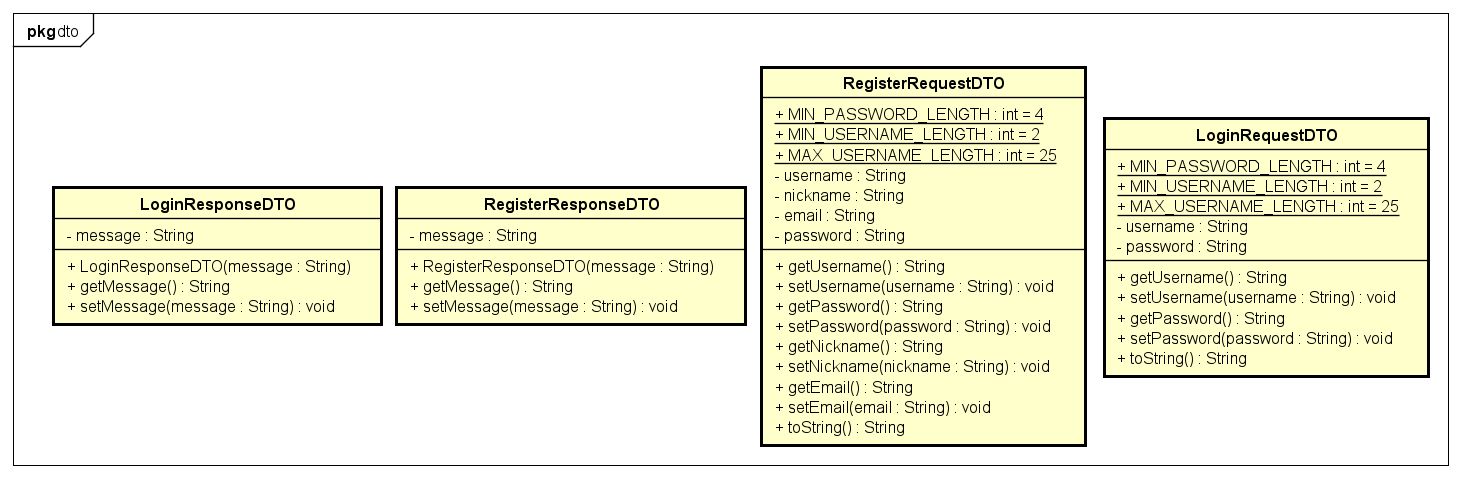
\includegraphics[width=\textwidth]{dijagrami/UML dtoovi.png}
				\caption{Dijagram razreda - dio DTO-ovi}
			\end{figure}
		
		    \begin{figure}[h]
		    	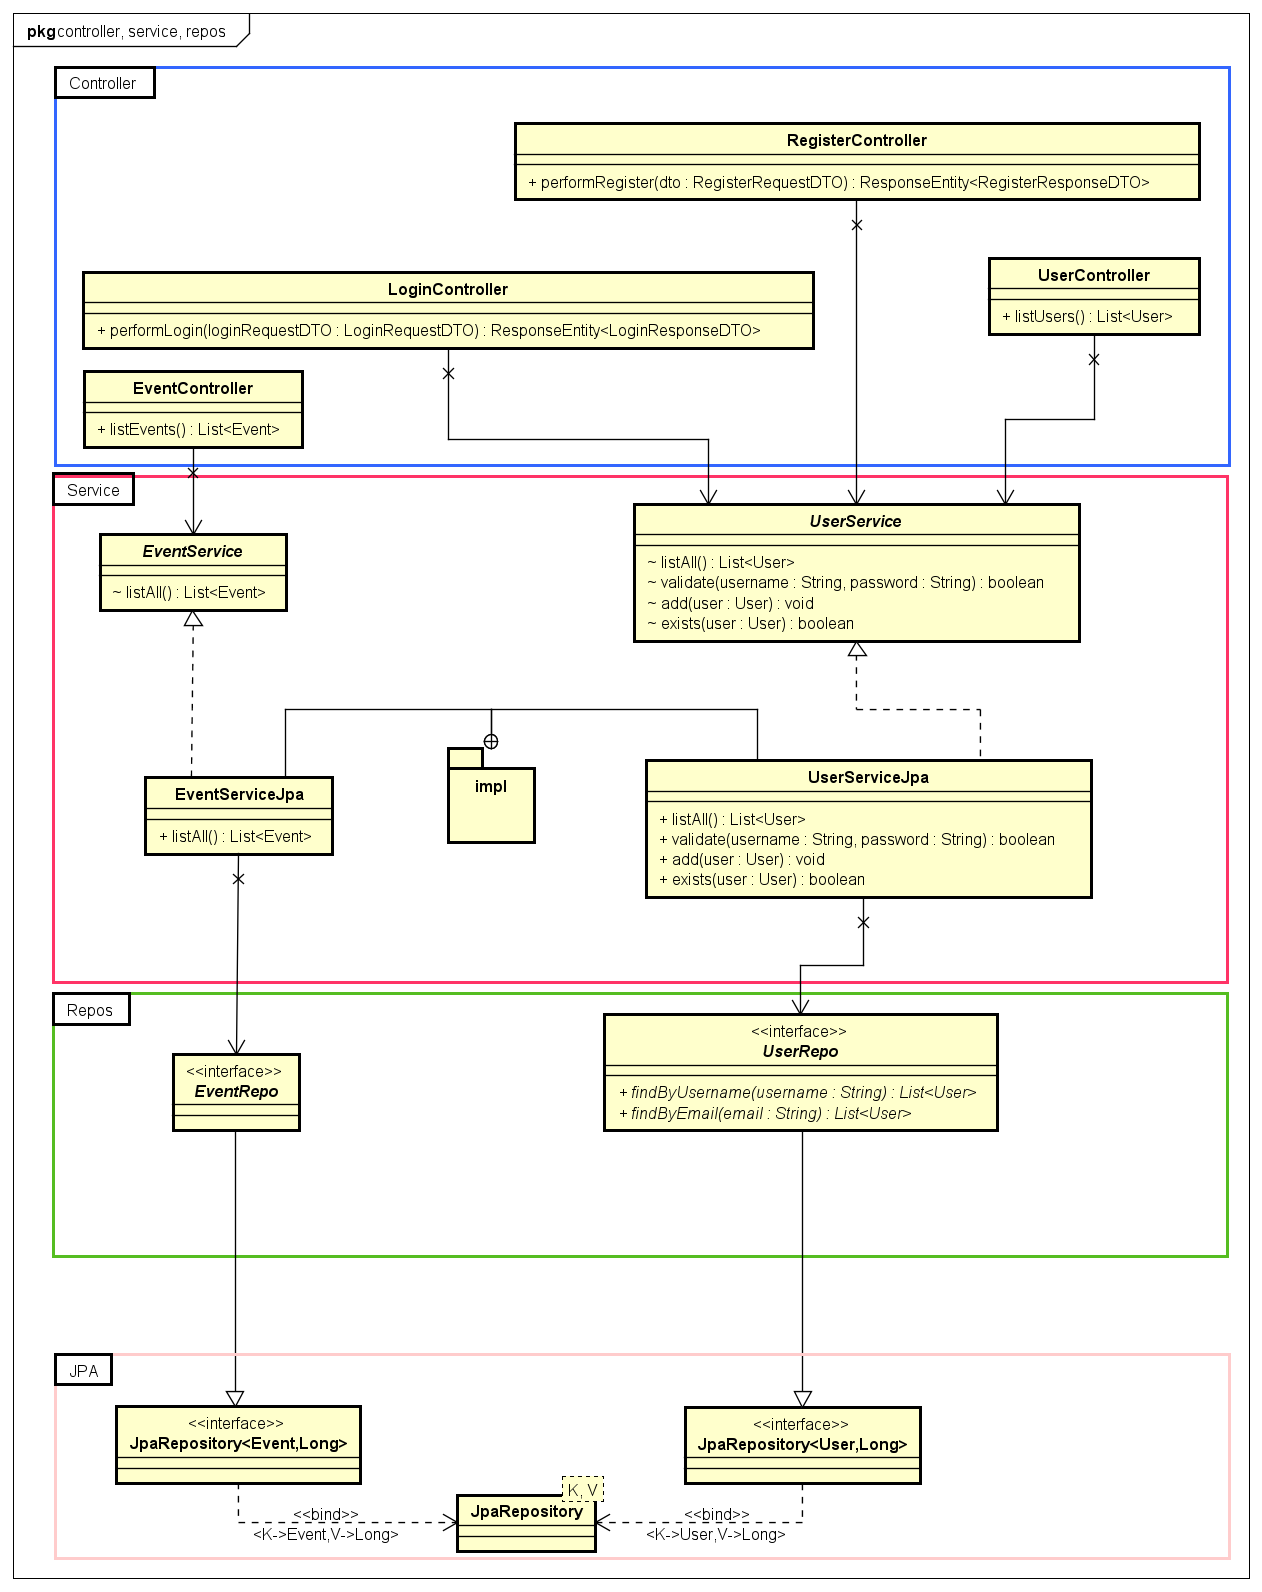
\includegraphics[width=\textwidth]{dijagrami/UML kontroleri, servisi, repozitoriji.png}
		    	\caption{Dijagram razreda - dio Kontroleri, servisi i repozitoriji}
		    \end{figure}
			
			\begin{figure}[h]
				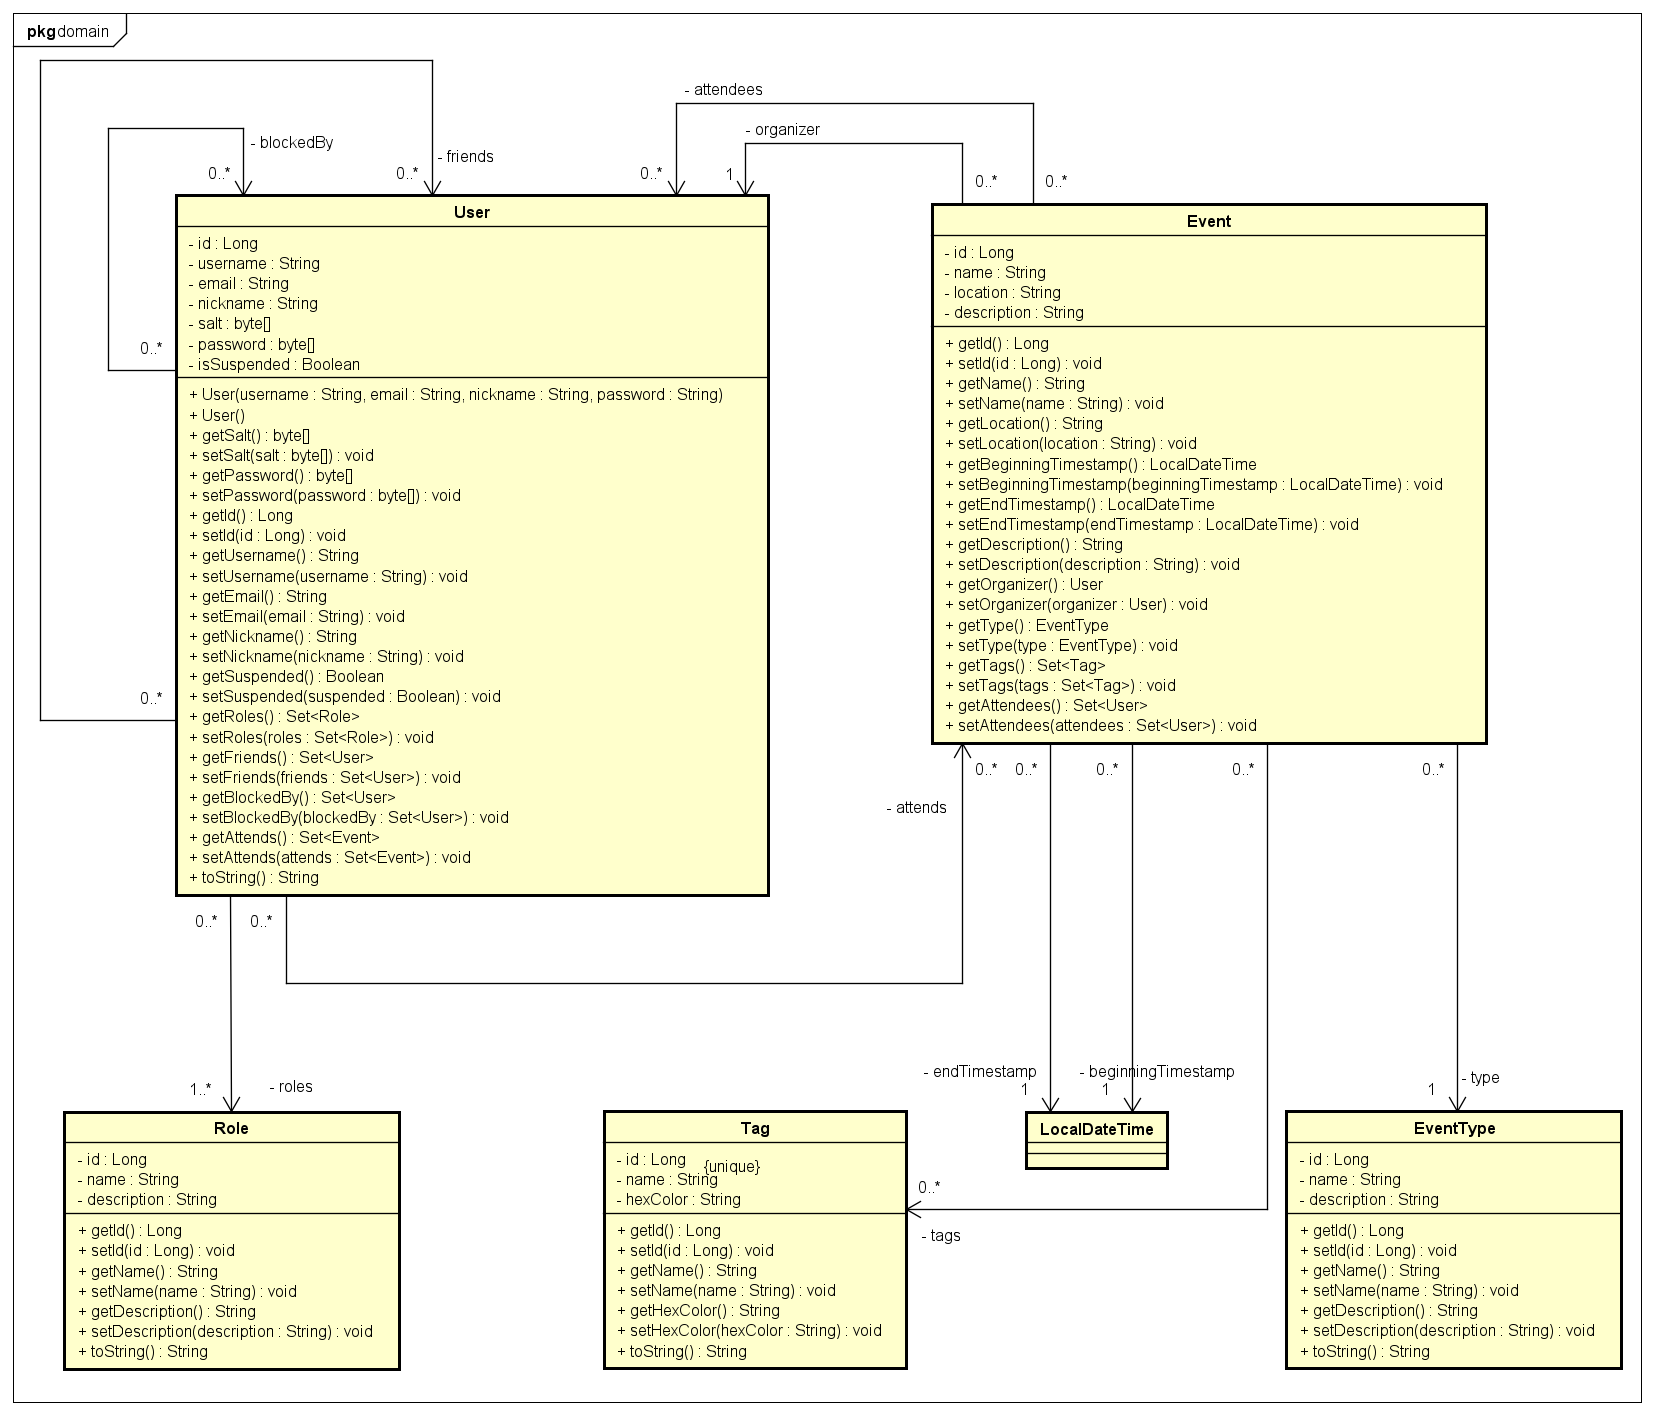
\includegraphics[width=\textwidth]{dijagrami/UML modeli.png}
				\caption{Dijagram razreda - dio Modeli}
			\end{figure}
		
			\eject
		
			\iffalse
			
				\textbf{\textit{dio 2. revizije}}\\			
			
				\textit{Prilikom druge predaje projekta dijagram razreda i opisi moraju odgovarati stvarnom stanju implementacije}
			
			
			
				\eject
		
			\section{Dijagram stanja}
			
			
				\textbf{\textit{dio 2. revizije}}\\
			
				\textit{Potrebno je priložiti dijagram stanja i opisati ga. Dovoljan je jedan dijagram stanja koji prikazuje \textbf{značajan dio funkcionalnosti} sustava. Na primjer, stanja korisničkog sučelja i tijek korištenja neke ključne funkcionalnosti jesu značajan dio sustava, a registracija i prijava nisu. }
			
			
				\eject 
		
			\section{Dijagram aktivnosti}
			
				\textbf{\textit{dio 2. revizije}}\\
			
			 	\textit{Potrebno je priložiti dijagram aktivnosti s pripadajućim opisom. Dijagram aktivnosti treba prikazivati značajan dio sustava.}
			
				\eject
			\section{Dijagram komponenti}
		
				\textbf{\textit{dio 2. revizije}}\\
		
			 	\textit{Potrebno je priložiti dijagram komponenti s pripadajućim opisom. Dijagram komponenti treba prikazivati strukturu cijele aplikacije.}
		\fi